\documentclass{article}
\usepackage[utf8]{inputenc}
\usepackage[top=3cm, bottom=3cm, left=3cm,right=3cm]{geometry}
%\usepackage[numbers,round]{natbib}
\usepackage{natbib}
\setcitestyle{aysep={}} 
\usepackage{graphicx}
\usepackage{color}
\usepackage{amsfonts, amsmath}
\usepackage{setspace}
\usepackage{amsmath}
\usepackage{mathtools}
\usepackage{bbm}
\usepackage{float}
\usepackage{hyperref}
\usepackage[super]{nth}

\parindent0cm
\parskip0.5cm
\hyphenpenalty=10000
\pretolerance=10000
\usepackage{lineno}

% Line numbering works around align environment without requiring paragraph break
\let\oldalign\align
\let\oldendalign\endalign
\renewenvironment{align}{\linenomathNonumbers\oldalign}{\oldendalign\endlinenomath}

\linenumbers

\makeatletter
\newcommand{\customlabel}[2]{
\protected@write \@auxout {}{\string \newlabel {#1}{{#2}{}}}}
\makeatother

%\renewcommand\footnote[2][]{\relax}

\begin{document}
{\Large Ancestry process for infectious disease outbreaks with superspreading}

%Journal target:  Journal of Theoretical Biology? Theoretical Population Biology?

\vspace*{2cm}
Xavier Didelot$^{1,2,*}$, Ian Roberts$^{2}$, ...

\vspace*{2cm}
$^1$ School of Life Sciences, University of Warwick, United Kingdom\\\\
$^2$ Department of Statistics, University of Warwick, United Kingdom\\\\
$^*$ Corresponding author. Tel: 0044 (0)2476 572827. Email: \verb+xavier.didelot@gmail.com+

\vspace*{2cm}
Running title: Ancestry for outbreaks with superspreading

\vspace*{2cm}
Keywords: infectious disease epidemiology modelling; offspring distribution; superspreading; outbreaks; lambda-coalescent model; multiple mergers

%\newpage
%\section*{Abstract}
%TODO

\newpage
\section{Introduction}

An outbreak of an infectious disease typically starts when a single or a small number
of infected individuals appear within a susceptible population. Each infected individual
may come in contact and infected each of the susceptible individuals, who will then
become infected in their turn and spread the disease further. Most infectious disease
modelling theory describes situations where the disease is at an equilibrium, when the number
of infected individuals is high and/or with a significant part of the population already infected
\citep{Anderson1991,keeling2008modeling}. 
Here however we focus on the early stages of an epidemic, where the number of 
infected individuals is small and the number of susceptibles relatively high and unchanging.
In this situation it is useful to think about the number of infections that each newly infected
individual is likely to cause, and the probabilistic distribution for this number is often called
the offspring distribution \citep{Grassly2008}. 
The mean of the offspring distribution is called the basic
reproduction number $R_0$ and has been given much attention especially since
it determines how likely the outbreak is to spread, and how much effort would be needed
to bring it under control \citep{fraserFactorsThatMake2004}. 

If we consider that all
individuals are infectious for the same duration and with the same infectiousness,
the offspring distribution is Poisson distributed with mean $R_0$, which means that the variance
of the offspring distribution is also $R_0$. We would then say that there is no transmission
heterogeneity. However, in practice there are many reasons why this may not be the case,
with some individuals being infectious for longer, or being more infectious than others, or 
having more contacts with susceptibles, or being less symptomatic and therefore less likely
to reduce contact numbers, etc. All these factors cause the offspring distribution to be more 
dispersed than it would otherwise be, that is to have a variance greater than its mean $R_0$. 
A frequent choice to capture this overdispersion is to model the offspring distribution
using a Negative-Binomial distribution with mean $R_0$ and dispersion parameter $r$
\citep{Lloyd-Smith2005,Grassly2008}. When $r$ is close to zero the variance is high compared to the mean,
whereas when $r$ is high the variance becomes close to the mean. This transmission heterogeneity
is often called superspreading, although this is perhaps misleading
as it is the rule rather than the exception of how infectious disease spread. Superspreading has
indeed been described in many diseases \citep{woolhouseHeterogeneitiesTransmissionInfectious1997,
steinSuperspreadersInfectiousDiseases2011,wangSuperspreadingHeterogeneityTransmission2021}, 
and most recently for 
SARS-CoV-2 \citep{Wang2020,lemieuxPhylogeneticAnalysisSARSCoV22021,gomez-carballaSuperspreadingEmergenceCOVID192021}.

As an outbreak unfolds forward-in-time, a transmission tree is generated representing who-infected-whom,
in which each node is an infected individual and points towards a number of nodes distributed according
to the offspring distribution. Here we consider the reverse problem of the transmission ancestry, going backward-in-time,
of a sample of infected individuals. 

\section{General case}

Let time be measured in discrete units and denoted $t$. Each discrete value of $t$ correspond to a unique non-overlapping 
generations of infected individuals, so that individuals infected at $t$ will have offspring at $t+1$, etc. 
Let $N_t$ denote the number of infectious individuals at time $t$. Each of them creates a number $s_{t,i}$ of secondary infections at time $t+1$, following the offspring distribution $\alpha_t(s)$. The mean of this distribution is the basic reproduction number $R_t$ and the variance is $V_t$. We have:

\begin{equation}
N_{t+1}=\sum_{i=1}^{N_t} s_{t,i}
\label{eq:summation}
\end{equation}

\subsection{Inclusive coalescence probability}

Inclusive coalescence probability $p_{k,t}(N_t, N_{t+1})$ is the probability that a specific set of $k$ individuals from generation $t+1$ find a common ancestor in generation $t$, conditional on population sizes $N_t$ and $N_{t+1}$.

Given full information about offspring counts from individuals in generation $t$ ${\bf s}_t = (s_{t,1}, \dots s_{t, N_t})$, we have

{\allowdisplaybreaks
	\begin{align}
		p_{k,t}({\bf s}_t, N_t)
			& = \sum_{i=1}^{N_t} \frac{\binom{s_{t,i}}{k}}{\binom{N_{t+1}}{k}} \nonumber\\
%			& = \sum_{i=1}^{N_t} \frac{s_{t,i}!}{(s_{t,i}-k)!} \frac{(N_{t+1}-k)!}{N_{t+1}!} \\
			& = \sum_{i=1}^{N_t} \frac{\Gamma(s_{t,i}+1) \Gamma(N_{t+1}-k+1)}{\Gamma(s_{t,i}-k+1) \Gamma(N_{t+1})}.% \\
%			& = \sum_{i=1}^{N_t} \frac{s_{t,i} (s_{t,i} - 1) \dots (s_{t,i} - k + 1)}{N_{t+1} (N_{t+1} - 1) \dots (N_{t+1} - k+1)}.
	\end{align}
}

Full information $\{s_{t,i}\}$ yields the population size $N_{t+1}$ but is not feasible to observe in practice.
We can instead express the inclusive coalescence probability conditioning on the next population size $N_{t+1}$ by summing over possible offspring counts ${\bf s}_t = (s_{t,1}, \dots s_{t, N_t})$ conditional on the total generation size.
Let $S_t^{-(1)} = (S_{t,2}, \dots, S_{t, N_t})$.

{\allowdisplaybreaks
	\begin{align}
	p_{k,t}(N_t, N_{t+1})
%		& = \sum_{{\bf s}_t : \sum_{i=1}^{N_t} s_{i,t} = N_{t+1}} 
		& = \sum_{{\bf s}_t \in \mathbb{N}_0^{N_t}} \mathbb{P} \bigg[{\bf S}_t = {\bf s}_t \bigg| \sum_{i=1}^{N_t} S_{t,i} = N_{t+1} \bigg] p_{k,t}({\bf s}_t, N_t) \nonumber\\
%		& = \sum_{{\bf s}_t : \sum_{i=1}^{N_t} s_{i,t} = N_{t+1}} 
		& = \sum_{{\bf s}_t \in \mathbb{N}_0^{N_t}} \mathbb{P} \bigg[{\bf S}_t = {\bf s}_t \bigg| \sum_{i=1}^{N_t} S_{t,i} = N_{t+1} \bigg] \sum_{i=1}^{N_t} \frac{\binom{s_{t,i}}{k}}{\binom{N_{t+1}}{k}} \nonumber\\
%		& = \sum_{i=1}^{N_t} \sum_{{\bf s}_t : \sum_{i=1}^{N_t} s_{i,t} = N_{t+1}} 
		& = \sum_{i=1}^{N_t} \sum_{{\bf s}_t \in \mathbb{N}_0^{N_t}}\frac{\binom{s_{t,i}}{k}}{\binom{N_{t+1}}{k}} \mathbb{P} \bigg[S_{t,1} = s_{t,1}, {\bf S}_t^{-(1)} = {\bf s}_t^{-(1)} \bigg| \sum_{i=1}^{N_t} S_{t,i} = N_{t+1} \bigg] \nonumber\\
		& = \frac{N_t}{\binom{N_{t+1}}{k}} 
%		\sum_{{\bf s}_t : \sum_{i=1}^{N_t} s_{i,t} = N_{t+1}}
		\sum_{{\bf s}_t \in \mathbb{N}_0^{N_t}} \binom{s_{t,1}}{k} \mathbb{P} \bigg[S_{t,1} = s_{t,1} \bigg| \sum_{i=1}^{N_t} S_{t,i} = N_{t+1} \bigg] \nonumber \\
			& \phantom{=}\qquad \times \mathbb{P} \bigg[{\bf S}_t^{-(1)} = {\bf s}_t^{-(1)} \bigg| S_{t,1} = s_{t,1}, \sum_{i=1}^{N_t} S_{t,i} = N_{t+1} \bigg] \nonumber\\
		& = \frac{N_t}{\binom{N_{t+1}}{k}} \sum_{s_{t,1} = 0}^{N_{t+1}} \binom{s_{t,1}}{k} \mathbb{P} \bigg[S_{t,1} = s_{t,1} \bigg| \sum_{i=1}^{N_t} S_{t,i} = N_{t+1} \bigg] \nonumber \\
			& \phantom{=}\qquad \times \underbrace{
				%\sum_{{\bf s}_t^{-(1)} : \sum_{i=2}^{N_t} s_{i,t} = N_{t+1} - s_{1,t}} 
				\sum_{{\bf s}_t^{-(1)} \in \mathbb{N}_0^{N_t - 1}} \mathbb{P} \bigg[{\bf S}_t^{-(1)} = {\bf s}_t^{-(1)} \bigg| \sum_{i=2}^{N_t} S_{t,i} = N_{t+1} - s_{1,t} \bigg]}_{=1} \nonumber\\
		& = \frac{N_t}{\binom{N_{t+1}}{k}} \mathbb{E}\bigg[ \binom{S_{t,1}}{k} \bigg| \sum_{i=1}^{N_t} S_{t,i} = N_{t+1} \bigg] \label{eq:GeneralInclusiveProb} %\nonumber\\
%		& = N_t \frac{(N_{t+1} - k)!}{N_{t+1}!} \mathbb{E} \bigg[ \frac{S_{t,1}!}{(S_{t,1} - k)!} \bigg | \sum_{i=1}^{N_t} S_{t,i} = N_{t+1} \bigg]. \label{eq:GeneralInclusiveProb}
	\end{align}
}

The falling factorial moments $\mathbb{E} \big[ \frac{S_{t,1}!}{(S_{t,1} - k)!} \big | \sum_{i=1}^{N_t} S_{t,i} = N_{t+1} \big]$ in Equation \eqref{eq:GeneralInclusiveProb} can be readily obtained by differentiating the probability generating function of $S_{t,1} | (\sum_{i=1}^{N_t} S_{t,i} = N_{t+1})$.

\subsection{Exclusive coalescence probability}

Generally, we observe a sample of individuals from each generation rather than the entire population.
In this case, we are interested in the exclusive coalescence probability $p_{n,k,t}(N_t, N_{t+1})$ that exactly $k$ individuals from a sample of $n$ arose from a common ancestor one generation in the past given knowlege of the total population sizes $N_t$ and $N_{t+1}$.

Given full information about offspring counts of the parents of sampled individuals at the present, ${\bf x}_t = (x_{t,1}, \dots, x_{t,N_t})$, we have
	\begin{align}
		p_{n,k,t}({\bf x}_t, N_t)
			& = \sum_{i=1}^{N_t} \frac{\binom{x_{t,i}}{k}}{\binom{n}{k}} \mathbb{I} \{ x_{t,i} = k \}\nonumber\\
			& = \sum_{i=1}^{N_t} \frac{x_{t,i}!}{(x_{t,i} - k)!} \frac{(n-k)!}{n!} \mathbb{I} \{ x_{t,i} = k \}.
	\end{align}

Similarly to the exclusive coalescence probability, we can use this to evaluate the exclusive probability given $N_t$ and $N_{t+1}$ by summing over possible parent offspring configurations (for $k \leq n$),

	\begin{align}
		p_{n,k,t}(N_t, N_{t+1})
			& = \sum_{{\bf x}_t \in \mathbb{N}_0^{N_t}} \mathbb{P} \bigg[ {\bf X}_t = {\bf x}_t \bigg | \sum_{i=1}^{n} X_{t,i} = n \bigg] p_{n,k,t} ({\bf x}_t, N_t) \nonumber\\
			& = \sum_{{\bf x}_t \in \mathbb{N}_0^{N_t}} \mathbb{P} \bigg[ {\bf X}_t = {\bf x}_t \bigg | \sum_{i=1}^{n} X_{t,i} = n \bigg] \sum_{i=1}^{N_t} \frac{\binom{x_{t,i}}{k}}{\binom{n}{k}} \mathbb{I} \{ x_{t,i} = k \} \nonumber\\
			& = \frac{N_t}{\binom{n}{k}} \sum_{{\bf x}_t \in \mathbb{N}_0^{N_t}} \binom{x_{t,1}}{k} \mathbb{P} \bigg[ {\bf X}_t = {\bf x}_t \bigg| \sum_{i=1}^{N_t} X_{t,i} = n \bigg] \mathbb{I} \{x_{t,1} = k \} \nonumber\\
			& = \frac{N_t}{\binom{n}{k}}
%				\sum_{{\bf x}_t^{-(1)} : \sum_{i=2}^n x_{t,i} = n-k} 
				\sum_{{\bf x}_t^{-(1)} \in \mathbb{N}_0^{N_t - 1}} \binom{k}{k} \mathbb{P}\bigg[X_{t,1} = k, {\bf X}_t^{-(1)} = {\bf x}_t^{-(1)} \bigg| \sum_{i=1}^{N_t} X_{t,i} = n \bigg] \nonumber\\
			& = \frac{N_t}{\binom{n}{k}} \mathbb{P}[X_{t,1} = k \bigg| \sum_{i=1}^{N_t} X_{t,i} = n \bigg]
%				\sum_{{\bf x}_t^{-(1)} : \sum_{i=2}^n x_{t,i} = n-k} 
				\underbrace{\sum_{{\bf x}_t^{-(1)} \in \mathbb{N}_0^{N_t - 1}} \mathbb{P}\bigg[{\bf X}_t^{-(1)} = {\bf x}_t^{-(1)} \bigg| \sum_{i=1}^{N_t} X_{t,i} = n, X_{t,1} = k \bigg]}_{=1} \nonumber\\
			& = \frac{N_t}{\binom{n}{k}} \mathbb{P} \bigg[ X_{t,1} = k \bigg| \sum_{i=1}^{N_t} X_{i,t} = n \bigg]. \label{eq:GeneralExclusiveProb}
	\end{align}

Note that $X_{t,i}$ does not follow the same offspring distribution as $S_{t,i}$.
$(X_{t,1}, \dots, X_{t, N_t})$ consists of $n$ individuals sampled from generation $t+1$ without replacement - there is no guarantee that all offspring from any given parent are included in the sample.

\subsection{Complementarity of exclusive coalescence probabilities}

If we consider one of the lines observed amongst a set of $n$, it can either remain uncoalesced
(with probability $p_{n1t}$) or coalesce in an event of size $k$ (with probability $p_{n,k,t}$) with any set of $k-1$ lines among the $n-1$ other lines, leading to the following complementarity equation: 

\begin{equation}
\sum_{k=1}^n \binom{n-1}{k-1} p_{n,k,t} =1
\end{equation}

We can show that it is indeed satisfied by the formula in Equation \eqref{eq:GeneralExclusiveProb}:

	\begin{align}
		\sum_{k=1}^n \binom{n-1}{k-1} p_{n,k,t}
			& = \sum_{k=1}^n \binom{n-1}{k-1} \frac{N_t}{\binom{n}{k}} \mathbb{P}\left[X_1 = k \bigg| \sum_{i=1}^{N_t} X_i = n\right] \nonumber\\
			& = \sum_{k=1}^n N_t \frac{k}{n} \mathbb{P}\left[X_1=k \bigg| \sum_{i=1}^{N_t} X_i = n\right] \nonumber\\
			& = \frac{N_t}{n} \sum_{k=0}^n k \mathbb{P}\left[X_1 = k \bigg| \sum_{i=1}^{N_t} X_i = n\right] 
			%\tag{lower limit $k=0$ makes no difference overall}
			\nonumber\\
			& = \frac{N_t}{n} \mathbb{E}\left[X_1 \bigg| \sum_{i=1}^{N_t} X_i = n \right] \nonumber\\
%			& = p_{1,t} (N_t, n) = 1 %\tag{see below}
%	\end{align*}
%	Taken from \href{https://math.stackexchange.com/questions/2508465/conditional-expectation-of-random-variable-given-a-sum}{stackexchange (link)}
%	\begin{align}
%		\mathbb{E}[X_1 | \sum_{i=1}^{N_t} X_i = n]
			& = \frac{1}{n} \sum_{i=1}^{N_t} \mathbb{E}\left[X_i \bigg| \sum_{i=1}^{N_t} X_i = n\right] %\tag{$X_i$ i.i.d.} 
			\nonumber\\
			& = \frac{1}{n} \mathbb{E}\left[ \sum_{i=1}^{N_t} X_i \bigg| \sum_{i=1}^{N_t} X_i = n\right] \nonumber\\%\tag{Swap expectation, sum \it (possibly questionable?)} \\
			& = 1%\frac{n}{N_t}
	\end{align}
	
\section{Poisson case}

Here the offspring distribution is $\alpha_t = \text{Poisson}(R_t)$.
In this case, we have 
	\begin{equation}
		\sum_{i=1}^{N_t} S_{t,i} \sim \text{Poisson}(N_t R_t),
	\end{equation}
and conditional distribution
{\allowdisplaybreaks
	\begin{align}
		\mathbb{P}\bigg[S_{t,1} = s \bigg| \sum_{i=1}^{N_t} S_{t,i} = N_{t+1} \bigg]
			& = \frac{\displaystyle\mathbb{P}\bigg[S_{t,1} = s, \sum_{i=1}^{N_t} S_{t,i} = N_{t+1} \bigg]}{\displaystyle\mathbb{P}\bigg[\sum_{i=1}^{N_t} S_{t,i} = N_{t+1} \bigg]} \nonumber\\
			& = \frac{\displaystyle\alpha_t (s) \, \mathbb{P}\bigg[ \sum_{i=2}^{N_t} S_{t,i} = N_{t+1} - s \bigg]}{\displaystyle\mathbb{P}\bigg[\sum_{i=1}^{N_t} S_{t,i} = N_{t+1} \bigg]} \nonumber\\
			& = \frac{\displaystyle\frac{R_t^s e^{-R_t}}{s!} \cdot \frac{((N_t - 1)R_t)^{N_{t+1} - s}}{(N_{t+1} - s)!}}{\displaystyle\frac{(N_t R_t)^{N_{t+1}} e^{-N_t R_t}}{N_{t+1}!}} \nonumber\\
			& = \binom{N_{t+1}}{s} \left( \frac{1}{N_t} \right)^s \left( 1 - \frac{1}{N_t} \right)^{N_{t+1} - s}, 
	\end{align}
}
that is
	\begin{equation}
		S_{t,1} \bigg| \left(\sum_{i=1}^{N_t} S_{t,i} = N_{t+1}\right) \sim \text{Binomial}\left(N_{t+1}, \frac{1}{N_t}\right).
	\end{equation}

The falling factorial moments of $X \sim \mathrm{Binomial}(n,p)$ are
\citep{Potts1953}:

\begin{equation}
	\mathbb{E}\left[\frac{X!}{(X-r)!}\right]=\binom{n}{r} p^r r!
\end{equation}

By injecting this formula into Equation \eqref{eq:GeneralInclusiveProb} 
we obtain the inclusive probability of coalescence for $k$ lines:
\begin{equation}
	\mathbb{E} \left[ \binom{S_{t,1}}{k} \bigg| \sum_{i=1}^{N_t} S_{t,i} = N_{t+1} \right]
		= \frac{1}{k!} \mathbb{E} \left[ \frac{S_{t,1}!}{(S_{t,1} - k)!} \bigg| \sum_{i=1}^{N_t} S_{t,i} = N_{t+1} \right]
		= \frac{1}{k!} \, \frac{N_{t+1}!}{(N_{t+1} - k)!} \left( \frac{1}{N_t} \right)^k.
\end{equation}

Consequently, the inclusive probability of coalescence for $k$ lines is
\begin{equation}
	p_{k,t}=\frac{1}{N_t^{k-1}}.\label{eq:PoisInclusiveProb}
\end{equation}

By injecting the probability mass function of a binomial distribution in Equation 
\eqref{eq:GeneralExclusiveProb} we deduce that 
the exclusive probability of coalescence for $k$ lines from a sample of $n$ $(n \geq k)$ is
	\begin{equation}
		p_{n,k,t} = \frac{(N_t-1)^{n-k}}{N_t^{n-1}}.\label{eq:PoisExclusiveProb}
	\end{equation}
	
It is interesting to note that neither the inclusive nor the exclusive coalescence probability
depend on the mean $R_t$ of the Poisson offspring distribution or the size $N_{t+1}$
of the population at time $t+1$.
The inclusive coalescent probability in Equation \eqref{eq:PoisInclusiveProb}
can also be obtained conceptually by considering
that among the $k$ lines, the first one has an ancestor with probability one, 
and the remaining $k-1$ need to have the same ancestor among a set of $N_t$ from
which they choose uniformly at random so that the probability of picking the same ancestor
is $1/N_t$. The exclusive coalescent probability in Equation \eqref{eq:PoisExclusiveProb} 
can be derived likewise by considering
that in addition to the above, each of the $n-k$ other lines need to choose a different
ancestor, which happens with probability $(N_t-1)/N_t$.

Figure \ref{fig:pois} illustrates the inclusive and exclusive coalescence probabilities for
the Poisson case for a set of size $k=1$ to $k=10$ amongst a total of $n=10$ observed
lines, in a population of size $N_t=10$, $N_t=20$ or $N_t=30$. 

\begin{figure}[!t]
\begin{center}
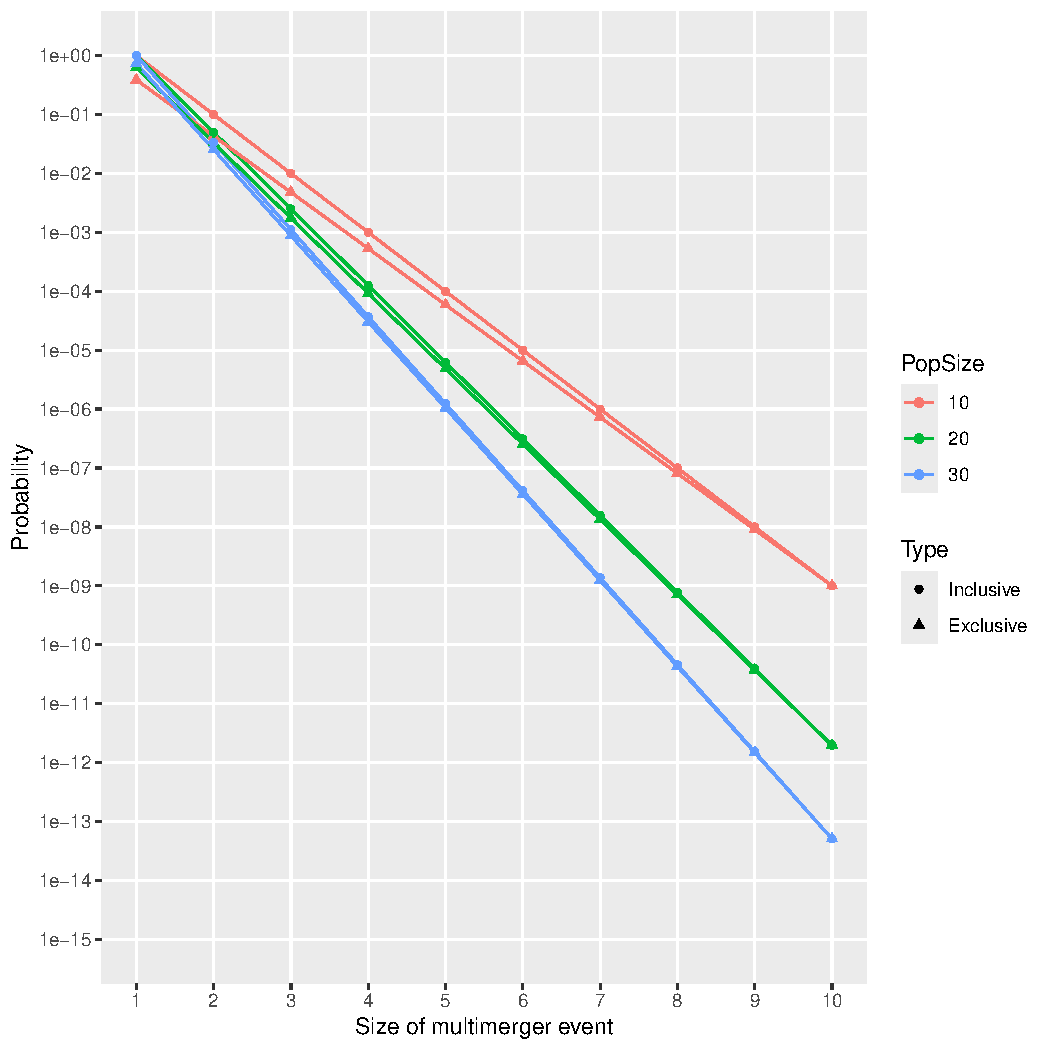
\includegraphics[width=15cm]{../run/figurePois.pdf}
\end{center}
\caption{Inclusive and exclusive coalescence probabilities for the Poisson case.
\label{fig:pois}}
\end{figure}

\section{Negative-Binomial case}

Here the offspring distribution is $\alpha_t=\text{Negative-Binomial}(r,p)$ with parameters $(r,p)$ set my moment-matching mean $R_t$ and variance $V_t$.
The resulting parameters for this distribution are $r=R_t^2/(V_t-R_t)$ and $p=R_t/V_t$.
In this case, we have
	\begin{equation}
		\sum_{i=1}^{N_t} S_{t,i} \sim \text{Negative-Binomial}(N_t r,p),
	\end{equation}
and similarly to the Poisson$(\lambda)$ offspring distribution identify the conditional distribution of $S_{t,1} | \sum_{i=1}^{N_t} S_{t,i}$ as follows,

{\allowdisplaybreaks
	\begin{align}
		\mathbb{P}\bigg[ S_{t,1} = s \bigg| \sum_{i=1}^{N_t} S_{t,i} = N_{t+1} \bigg]
			& = \frac{\alpha_t(s) \cdot \mathbb{P} \bigg[\sum_{i=2}^{N_t} S_{t,i} = N_{t+1} - s \bigg]}{\mathbb{P}\bigg[\sum_{i=1}^{N_t} S_{t,i} = N_{t+1} \bigg]} \nonumber\\
			& = \frac{\displaystyle\frac{\Gamma(r+s)}{s! \Gamma(r)} (1-p)^s p^r \cdot \frac{\Gamma\big((N_t - 1)r+(N_{t+1} - s)\big)}{(N_{t+1} - s)! \Gamma((N_t - 1) r)} (1-p)^{N_{t+1} - s} p^{(N_t-1)r}}{\displaystyle\frac{\Gamma(N_tr+N_{t+1})}{N_{t+1}! \Gamma(N_t r)} (1-p)^{N_{t+1}} p^{N_t r}} \nonumber\\
			& = \frac{N_{t+1}!}{s! (N_{t+1} - s)!} \frac{\Gamma(r+s) \Gamma\big( (N_t - 1)r + (N_{t+1} - s) \big)}{\Gamma(N_t r + N_{t+1})} \frac{\Gamma(N_t r)}{\Gamma(r) \Gamma\big((N_t - 1)r \big)} \nonumber\\
			& = \binom{N_{t+1}}{s} \frac{\mathrm{B}(s + r, N_{t+1} - s + (N_t-1)r)}{\mathrm{B}(r, (N_t-1)r)},
	\end{align}
}
that is $S_{t,1} \bigg| \bigg(\sum_{i=1}^{N_t} S_{t,i} = N_{t+1} \bigg) \sim \text{Beta-Binomial}(r, (N_t - 1)r)$.

The falling factorial moments of $X \sim \text{Beta-Binomial}(\alpha,\beta)$ are \citep{Tripathi1994}:

\begin{equation}
	\mathbb{E}\left[\frac{X!}{(X-r)!}\right]=\binom{n}{r} \frac{\mathrm{B}(\alpha+r,\beta)r!}{\mathrm{B}(\alpha,\beta)}
\end{equation}

\noindent where  $\mathrm{B}(x,y)$ denotes the Beta function defined as $\mathrm{B}(x,y)=\Gamma(x)\Gamma(y)/\Gamma(x+y)$, and injecting this formula into Equation \eqref{eq:GeneralInclusiveProb}, we deduce that the inclusive probability of coalescence for $k$ lines is:

\begin{equation}
p_{k,t}=
%\prod_{i=1}^{k-1}\frac{r+i}{N_t r+i}=
\frac{\mathrm{B}(N_t r+1,r+k)}{\mathrm{B}(r+1,N_t r+k)}
\label{eq:NegBinInclusiveProb}
\end{equation}

By injecting the probability mass function of a beta-binomial distribution in Equation 
\eqref{eq:GeneralExclusiveProb} we deduce that 
the exclusive probability of coalescence for $k$ lines is:

\begin{equation}
p_{n,k,t}=\frac{N_t \mathrm{B}(k+r, n-k+N_t r-r)}{\mathrm{B}(r, N_t r-r)}
\label{eq:NegBinExclusiveProb}
\end{equation}

It is interesting to note that as for the Poisson case, the inclusive and exclusive coalescence probabilities do not depend on the size $N_{t+1}$ of the population at time $t+1$.
They both depend on the 
Negative-Binomial offspring distribution only through the dispersion parameter $r$.

Figure \ref{fig:negbin} illustrates the inclusive and exclusive coalescence probabilities for
the Negative-Binomial case for a set of size $k=1$ to $k=10$ amongst a total of $n=10$
 observed lines, in a population of size $N_t=12$. 
Several Negative-Binomial offspring distributions are compared, 
all of which have the same mean $R_t=2$,
and with the dispersion parameter equal to $r=1$, $r=2$, $r=10$ and $r=100$.
When $r=1$ the Negative-Binomial reduces to a Geometric distribution.
When $r$ is high (for example $r=100$ as shown in Figure \ref{fig:negbin}) 
the dispersion is low and the Negative-Binomial case 
behaves almost like the Poisson case. When $r$ is lower the dispersion of the
offspring distribution increases, so that 
both the inclusive and exclusive probabilities of larger multimerger events increase.

\begin{figure}[!t]
\begin{center}
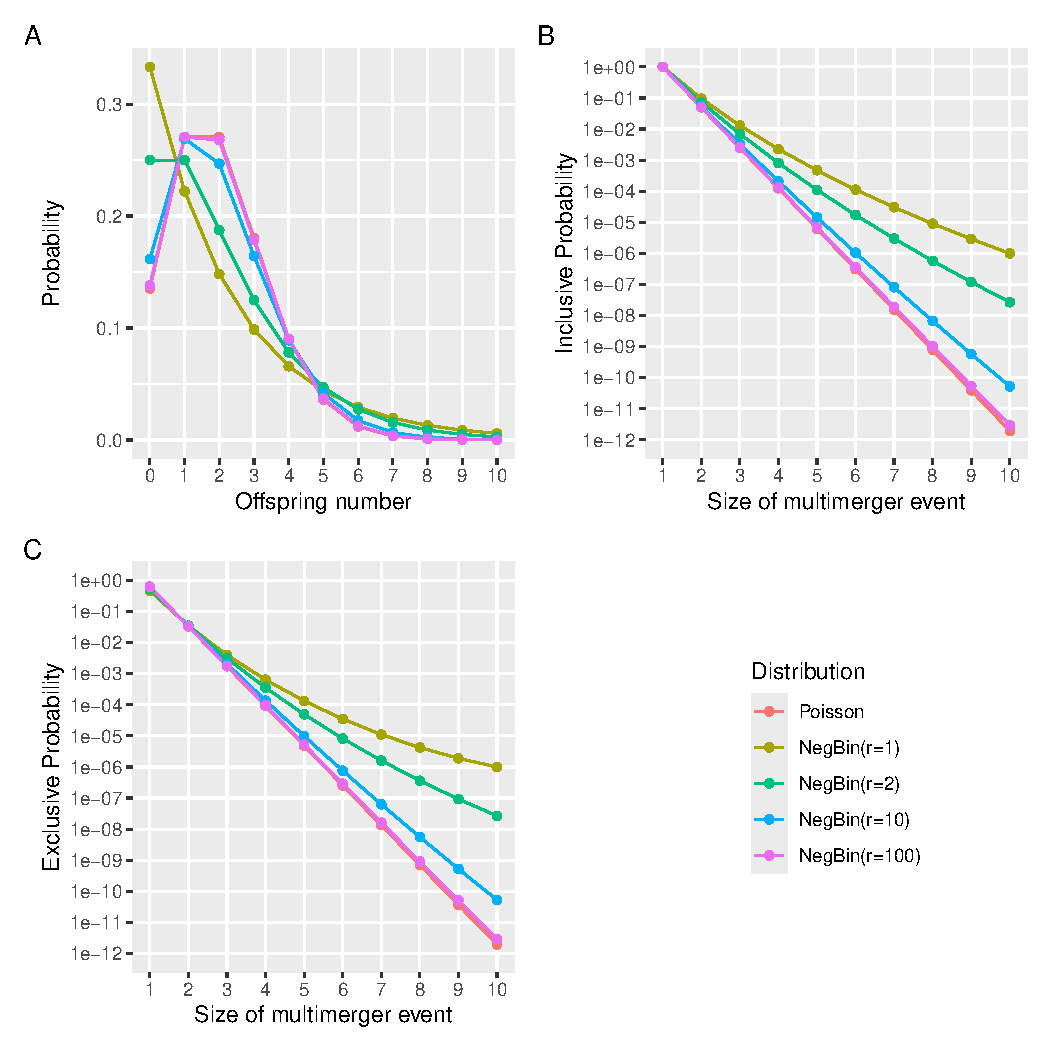
\includegraphics[width=15cm]{../run/figureNegBin.pdf}
\end{center}
\caption{(A) Offspring distribution. (B) Inclusive probability of coalescence. (C) Exclusive probability of coalescence.
\label{fig:negbin}}
\end{figure}

\section{Limit when the population size is large}

Consider that $N_t$ is large. 

Show that inclusive probabilities $p_{k,t}$ for $k>2$ are small compared to $p_{2,t}$.

Show that exclusive probabilities $p_{n,k,t}$ for $k>2$ is small compared to $p_{n,2,t}$, when $n<<N_t$.

Show that inclusive and exclusive probabilities become equal, when $n<<N_t$ in exclusive probabilities.

For Poisson offspring distribution we have:

\begin{equation}
p_{2,t}=p_{n,2,t}=\frac{1}{N_t}\label{eq:poissonapprox}
\end{equation}

For Negative-Binomial offspring distribution we have:

\begin{equation}
p_{2,t}=p_{n,2,t}=\frac{r+1}{N_t r +1} \approx \frac{r+1}{N_t r}\label{eq:negbinapprox}
\end{equation}

\citet{Fraser2017} calculated the effective population size $N_e(t)$ 
as a function of the actual population size $N(t)$ and the mean and variance of the offspring distribution $R$ and $\sigma^2$:
\begin{equation}
N_e(t)=\frac{N(t)}{\sigma^2/R+R-1}
\end{equation}

This formula was used to estimate the dispersion parameter from genetic data \citep{Li2017}.
In our notation, this is equivalent to:

\begin{equation}
 p_{2,t}=\frac{V_t/R_t+R_t-1}{N_t R_t}\label{eq:fraser}
 \end{equation}

In the Poisson case we have $V_t=R_t$ so that Equation \eqref{eq:fraser} simplifies to $p_{2,t}=1/N_t$ which agrees with Equation \eqref{eq:poissonapprox}. 
In the Negative-Binomial case we have $V_t/R_t=1/p=(r+R_t)/r$ so that Equation \eqref{eq:fraser}
simplifies to $(r+1)/(rN_t)$ which agrees with our Equation \eqref{eq:negbinapprox}. 
Conversely, if we substitute $r=R_t^2/(V_t-R_t)$
in Equation \eqref{eq:negbinapprox} we obtain the formula Equation \eqref{eq:fraser}.

\citet{koelleRatesCoalescenceCommon2012} derived the rates of coalescence of two lineages 
for several epidemiological models, assuming a large population at equilibrium.
For each model they use the equation $N_e=N/\sigma^2$ to relate the effective population
size $N_e$ to the actual population size $N$ and the variance $\sigma^2$ in the number
of offspring. This relationship was first established by \citet{Kingman1982} to
apply the coalescent model to Cannings exchangeable models. 
From Equation \eqref{eq:negbinapprox} we can take $R_t=1$ to achieve 
equilibrium of the population size and $r=R_t^2/(V_t-R_t)=1/(V_t-1)$ to deduce 
the equivalent $p_{2,t}=V_t/N_t$. 

\citet{Volz2012a} showed that the rate of coalescence for two lineages under a continuous-time epidemic coalescent model is $2f(t)/I(t)^2$
 where $f(t)$ is the incidence and $I(t)$ the prevalence. 
 Setting in this formula the prevalence as $I(t)=N_{t+1}=N_t R_t$ and the incidence as
 $f(t)=R_t N_{t+1}=R_t^2 N_t$ we get a coalescent rate of 
 $2/N_t$. To apply the Equation \eqref{eq:negbinapprox} we need to set $r=1$ 
 so that the offspring distribution is Geometric, which yields the same result.

\section{Lambda-coalescent}

The coalescent model \citep{Kingman1982,Kingman1982a} describes the ancestry of a sample from a large population 
evolving according to many forward-in-time models such as the Wright-Fisher model \citep{Wright1931,Fisher1930}, 
the Moran model \citep{Moran1958} and the Cannings exchangeable model \citep{Cannings1974}.
Since the coalescent considers a large population in which each individual only has a number of offspring that is small
compared to the population size, coalescent trees are always binary and do not feature multimergers,
making them unsuitable to represent the ancestry of outbreaks considered in this study.
However, the lambda-coalescent models are an extension of the coalescent model that do
allow multimergers
\citep{pitmanCoalescentsMultipleCollisions1999,sagitovGeneralCoalescentAsynchronous1999,donnellyParticleRepresentationsMeasureValued1999}. 

A lambda-coalescent model is defined by a probability measure 
$\Lambda(\mathrm{d} x)$ on the interval $[0,1]$, from which we can deduce
the rate $\lambda_{n,k}$ at which any subset of $k$ lineages within a set of $n$ observed lineages 
coalesce:

\begin{equation}
    \lambda_{n,k} = \int_{0}^{1}{x^{k-2}(1-x)^{n-k}\,\Lambda(\mathrm{d} x)}
\end{equation}

The beta-coalescent \citep{schweinsbergCoalescentProcessesObtained2003} is a specific type of Lambda-coalescent. 
Was used in \citep{Hoscheit2019} and \citep{Menardo2021}. 
David's paper on inference of multiple mergers while dating a pathogen phylogeny \citep{Helekal2024}.

The Beta$(2-\alpha,\alpha)$-coalescent model \citep{schweinsbergCoalescentProcessesObtained2003}
has a single parameter $\alpha \in [0,2]$ and is defined as:

\begin{equation}
\Lambda(\mathrm{d}x)=\frac{x^{1-\alpha}(1-x)^{\alpha-1}}{\mathrm{B}(2-\alpha,\alpha)}\mathrm{d}x
\end{equation}

from which we can deduce that:

\begin{equation}
\lambda_{n,k}=\frac{\mathrm{B}(k-\alpha,n-k+\alpha)}{\mathrm{B}(2-\alpha,\alpha)}
\end{equation}

Special cases include $\alpha=2$ corresponding to the Kingman coalescent,
$\alpha=1$ which is known as the Bolthausen-Sznitman coalescent
and $\alpha=0$ for which the phylogeny is always star-shaped.

The exclusive coalescent probability in the Negative-Binomial case 
(Equation \ref{eq:NegBinExclusiveProb}) could be used as the $\lambda_{n,k}$.
Figure \ref{fig:tree} shows an example with $n=20$, $N_t=40$ and $r=0.5$.

\begin{figure}[!t]
\begin{center}
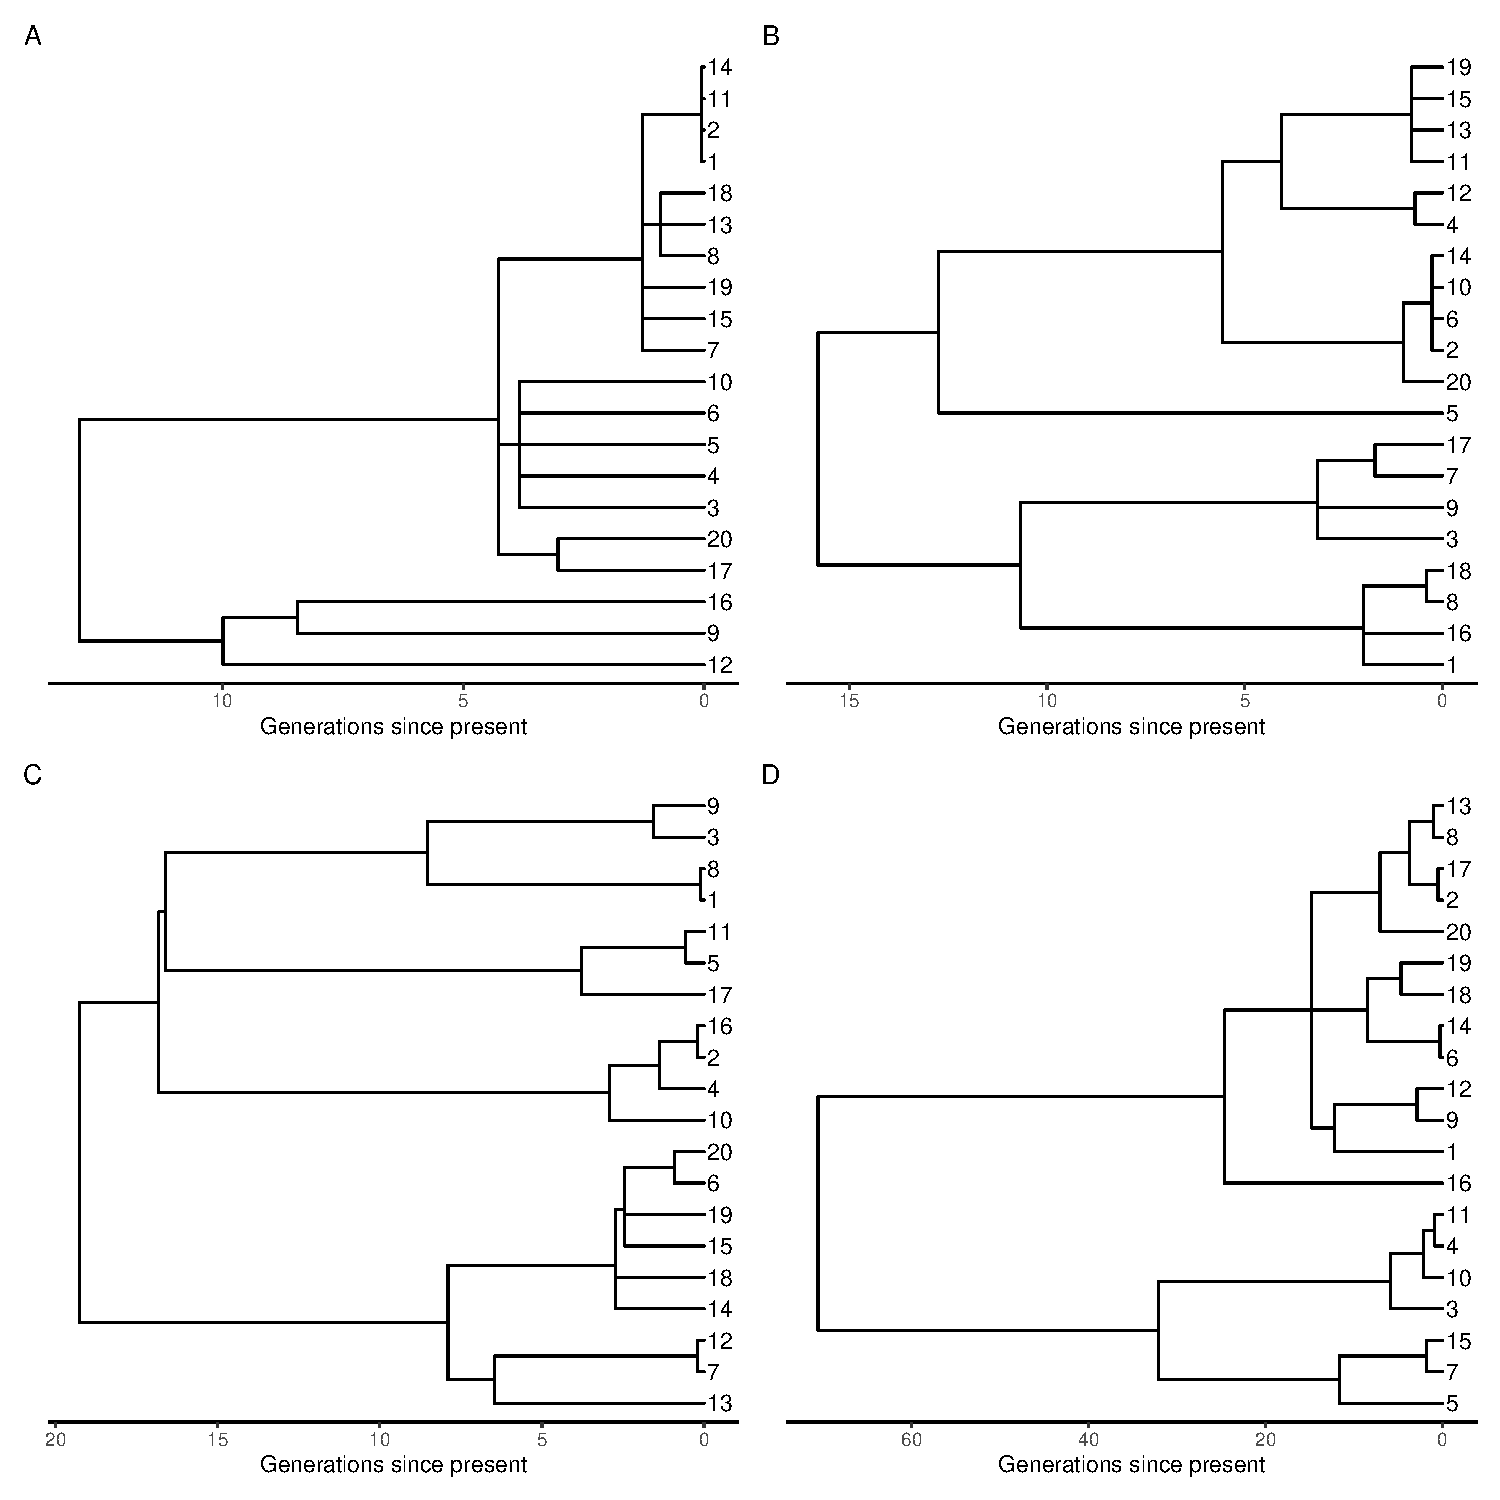
\includegraphics[width=15cm]{../run/figureTree.pdf}
\end{center}
\caption{Tree example
\label{fig:tree}}
\end{figure}


\section{Implementation}

We implemented the analytical methods described in this paper in a 
new R package entitled \emph{EpiLambda} which is available
at \url{https://github.com/xavierdidelot/EpiLambda} for R version 3.5 or later. 
All code and data needed to replicate the results are included in the ``run'' directory of the \emph{EpiLambda} repository.

\section{Discussion}

Either here of before discuss the Xi-coalescent models which admit multiple 
simultaneous mergers \citep{schweinsbergCoalescentsSimultaneousMultiple2000}.

\section*{Acknowledgements}

We acknowledge funding from the National Institute for Health Research (NIHR) Health Protection Research Unit in Genomics and Enabling Data.

\newpage
\bibliographystyle{elsarticle-harv}
%\bibliography{biblio,/Users/u1775021/all.bib}
\bibliography{biblio}

\end{document}

